\documentclass{report}

% Packages
\usepackage[utf8]{inputenc}
\usepackage{amsmath}
\usepackage{amssymb}
\usepackage{amsthm}
\usepackage{graphicx}
\usepackage{float}
\usepackage{hyperref}
\usepackage{url}
\usepackage[strings]{underscore}
\usepackage{listings}

% All in preamble:

\usepackage{listings}
\usepackage{courier}
\usepackage{color}

\definecolor{mygreen}{rgb}{0,0.6,0}
\definecolor{mygray}{rgb}{0.5,0.5,0.5}
\definecolor{mymauve}{rgb}{0.58,0,0.82}
\lstset{ %
  backgroundcolor=\color{white},   % choose the background color; you must add \usepackage{color} or \usepackage{xcolor}
  basicstyle=\footnotesize\ttfamily,        % the size of the fonts that are used for the code
  breakatwhitespace=false,         % sets if automatic breaks should only happen at whitespace
  breaklines=true,                 % sets automatic line breaking
  captionpos=b,                    % sets the caption-position to bottom
  commentstyle=\color{mygreen},    % comment style
  deletekeywords={...},            % if you want to delete keywords from the given language
  escapeinside={\%*}{*)},          % if you want to add LaTeX within your code
  extendedchars=true,              % lets you use non-ASCII characters; for 8-bits encodings only, does not work with UTF-8
  frame=single,                    % adds a frame around the code
  keepspaces=true,                 % keeps spaces in text, useful for keeping indentation of code (possibly needs columns=flexible)
  keywordstyle=\color{blue},       % keyword style
  language=Python,                 % the language of the code
  otherkeywords={*,...},            % if you want to add more keywords to the set
  numbers=left,                    % where to put the line-numbers; possible values are (none, left, right)
  numbersep=5pt,                   % how far the line-numbers are from the code
  numberstyle=\tiny\color{mygray}, % the style that is used for the line-numbers
  rulecolor=\color{black},         % if not set, the frame-color may be changed on line-breaks within not-black text (e.g. comments (green here))
  showspaces=false,                % show spaces everywhere adding particular underscores; it overrides 'showstringspaces'
  showstringspaces=false,          % underline spaces within strings only
  showtabs=false,                  % show tabs within strings adding particular underscores
  stepnumber=2,                    % the step between two line-numbers. If it's 1, each line will be numbered
  stringstyle=\color{mymauve},     % string literal style
  tabsize=2,                       % sets default tabsize to 2 spaces
  title=\lstname                   % show the filename of files included with \lstinputlisting; also try caption instead of title
}


\hypersetup{
    colorlinks=true,
    linkcolor=blue,
    filecolor=magenta,      
    urlcolor=cyan,
    pdftitle={Overleaf Example},
    pdfpagemode=FullScreen,
}

\begin{document}

\begin{titlepage}
    \begin{center}
        \vspace*{1cm}
 
        \Large\textbf{Reinforcement Learning: Combates de Pokémon }
 
        \vspace{0.5cm}
	Antecedentes, implementación y resultados
             
        \vspace{1.5cm}
	    \textbf{Alejandro Jiménez, Alejandro Gómez, Luis Crespo y Antonio Cabrera} 

        \vfill
             
        Trabajo para el doble grado de\\
        Ingeniería del Software y Matemática Computacional\\
             
        \vspace{0.8cm}
      
        
\includegraphics[width=0.4\textwidth]{figures/logo u-tad.png}
             
        Asignatura de inteligencia artifial\\
        U-tad\\
        España\\
        Enero 2024
             
    \end{center}
 \end{titlepage}

\tableofcontents
\listoffigures

\chapter{Introducción}

\section{Contexto}

Desde que Deep Blue gana a Kasparov en 1997, las máquinas han ido superando a los humanos en la mayoría de juegos clásicos. Con los avances en computación y en Deep Learning la diferencia entre los grandes maestros y los ordenadores es más grande que nunca. La nueva generación de bots para jugar a juegos hace uso del Reinforcement Learning, que consiste en entrenar a una red neuronal en base a lo que aprende jugando contra ella misma.

Pokémon es la franquicia de entretenimiento más grande del mundo, con más de 300 millones de juegos vendidos. El juego consiste en capturar criaturas llamadas Pokémon y entrenarlos para que luchen contra otros Pokémon. A pesar de que el juego fue pensado para niños, Pokémon cuenta con una escena competitiva muy profesional (el torneo mundial de 2024 contará con 2.000.000 de euros en premios), sin embargo el uso de inteligencias artificiales aun no se ha extendido como en otros juegos.

\section{Objetivos}
El objetivo de este trabajo es crear un bot que sea capaz de jugar a Pokémon de forma autónoma. Para ello se ha utilizado una versión simplificada del juego programada en python, en la que se eliminan ciertos elementos como el azar en la partida. El bot se ha entrenado utilizando el algoritmo de Reinforcement Q-Learning , haciendo uso de la librería de PyTorch.



\chapter{Explicación del juego}

\section{Batallas}

El juego se basa en batallas entre dos jugadores, cada uno cuenta con un equipo de 6 pokémon, de los cuales solo puede tener uno en el campo de batalla. 
\subsection{Turnos}
El juego se divide en turnos, en cada turno el jugador puede realizar una acción, ya sea atacar, cambiar de pokémon. Al comienzo de cada turno ambos jugadores selecciona una acción, en el caso de que ambos decidan atacar atacará primero el pokémon con más velocidad. 

\begin{figure}[H]
        \centering
        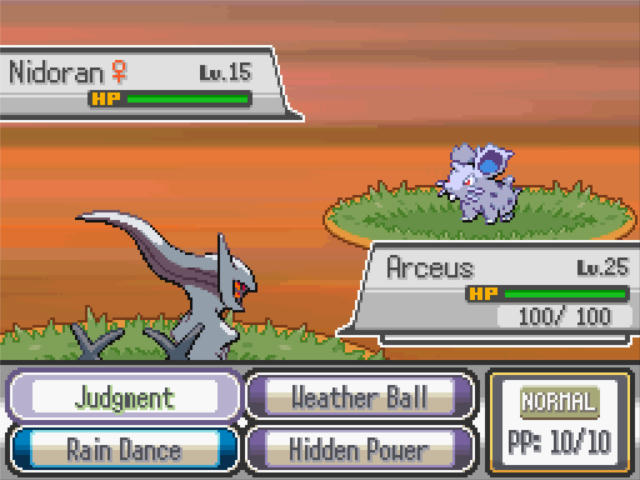
\includegraphics[width=0.5\textwidth]{figures/combat.jpg}
        \caption{Jugador eligiendo el ataque de su pokémon.}
        \label{fig:turn}
\end{figure}

\chapter{Reinforcement Learning}

A continuación, se va a explicar brevemente en qué consiste el Reinforcement Learning (a partir de ahora RL), además de explicar cómo se aplicará este area del aprendizaje automático a nuestro trabajo.

El RL es un paradigma de aprendizaje automático que se centra en enseñar a un agente a tomar decisiones secuenciales para maximizar una recompensa acumulativa a lo largo del tiempo. En este enfoque de aprendizaje automático, el agente interactúa con un entorno dinámico y aprende a base de las recompensas y penalizaciones que conllevan sus decisiones.

\section{Reinforcement Learning aplicado a Pokémon}

Como en este trabajo estamos llevando a cabo batallas pokemon, el agente tiene un rango de 4 opciones a la hora de realizar una accion. Estas opciones son los 4 movimientos que puede efectuar el pokemon que está en ese momento luchando. La forma en la que se entregarán recompensas y penalizaciones al agente será en base de si estos movimientos inflingen daño (quitan puntos de vida del pokemon al que se enfrenta), o si gana el combate. De esta forma el agente aprenderá qué movimientos son los óptimos para los distintos pokemons.

El agente también posee un estado, en relación con el entorno de este trabajo. Este estado incluirá valores como, por ejemplo, el tipo o tipos de Pokémon que el agente maneja y el Pokémon al que se enfrenta, las puntuaciones de vida de los Pokémon y los movimientos disponibles de los Pokémon.

Para elegir la accion que realizará el Pokémon, el modelo que se creará tendrá que recibir como inputs, todos los valores del estado comentados previamente y devolvera un output de 4 valores correspondientes a los 4 posibles movimientos del Pokémon controlado por el agente, de los cuales se elegirá el que tenga un mayor valor.

\section{Deep Q-Learning}

Este trabajo tambien va a estar centrado en Deep Q-Learning, un enfoque en el campo del deep learning aplicado a la toma de decisiones en entornos dinámicos como el que estamos usando. Q-Learning es un algoritmo que buscan aprender una función Q con la que evaluar la calidad de las acciones en un estado dado.

Para esto vamos a tener que implementar una red neuronal profunda para evitar utilizar tablas con todas las posibles combinaciones de acciones y estados, que en este caso serían tablas de proporciones demasiado grandes teniendo en cuenta todos los movimientos, pokemons y tipos que se han comentado anteriormente. 

La función Q es una función que asigna un valor para cada par estado-acción y se denota como Q(s,a), donde s respresenta el estado y a la acción. Esta función representa el valor esperado de tomar una acción en un estado especfíco, es decir, mide cuánto valor acumulativo (de recompensas) se espera obtener de realizar dicha acción es ese estado, y de esta forma saber cuál es la estrategia que seguir de ahí en adelante.

El Q-Learning presenta un algoritmo para entrenar al agente en el entorno propuesto, y sigue los siguientes pasos:
\begin{enumerate}
	\item Inicialización
		\begin{itemize}
			\item Inicializa la función Q(s,a) de forma arbitraria para todos los pares estado-	acción.\newline
			\item Establece los parámetros del algoritmo: tasa de aprendizaje, factor de descuento y 	otros que se explicarán más adelante.\newline
		\end{itemize}

	\item Exploración/ Explotación (Realizar acciones)
		\begin{itemize}
			\item En cada frame o etapa del proceso, se elige una acción a realizar en el estado 	actual. Esta decisión puede ser determinista o estocástica, la primera se basa en 	elegir la acción que tiene el mayor valor Q conocido (explotacion), mientras que la 	segunda busca realizar acciones nuievas para descubrir como de efectivas o útiles son 	(exploración).
		\end{itemize}

	\item Interaccion con el entorno
		\begin{itemize}
			\item Una vez la acción ha sido realizada, se observa la recompensa o penalización 	recibida y el próximo estado.
	    \end{itemize}

	\item Actualización de la función Q
		\begin{itemize}
			\item Se usa la ecuación de Bellman para actualizar Q(s,a):
		\end{itemize}
		\begin{equation}
		Q(s, a) \leftarrow Q(s, a) + \alpha \cdot \left[ r + \gamma \cdot \max_{a'} 		Q(s', a') - Q(s, a) \right]
		\end{equation}

		Donde:
		\begin{itemize}
			\item(alpha) es la tasa de aprendizaje que controla la magnitud de la actualización.
			\item r es la recompensa obtenida
			\item gamma como el factor de descuento que penaliza las recompensas a largo plazo.
			\item max_a'Q(s',a') representa el valor máximo esperado en el proximo estado s'
		\end{itemize}

	\item Repetición
		\begin{itemize}
			\item Se realizan los pasos del 2 al 4 durante un número de frames o iteraciones.
		\end{itemize}

	\item Convergencia
		\begin{itemize}
			\item La función Q converge a la función de valor óptimo a medida que el agente explora 	y aprende mas sobre el entorno.
		\end{itemize}

	\item Política óptima
		\begin{itemize}
			\item La política óptima se obtiene a partir de la función Q resultante, la acción 	óptima es aquella que maximiza Q(s,a).
		\end{itemize}
\end{enumerate}
Este algoritmo es un proceso iterativo en el que el agente interactúa con el entorno y cambia sus estimaciones de Q, de esta forma creando una política o estrategia para maximizar las recompensas. Un equilibrio entre la exploración y la explotación es de gran importancia para asegurar que el agente conoce las mejores acciones a realizar sin atascarse en comportamientos subóptimos.

\chapter{IA Pokemon}

Habiendo establecido el funcionamiento del RL y del Deep Q-Learning, se explicará como se aplican al entrenamiento de una IA capaz de realizar batallas pokemon.

\section{Entorno}

El entorno del que se ha hablado anteriormente tiene un rol de suma importancia pues al programar este en la clase "environment.py", se le ha añadido la función "step()". Esta funcion es la encargada de dirigir las batallas pokemon pues elige el movimiento del pokemon, ejecuta el turno y calcula las recompensas a impartir en los agentes, que son los dos contrincantes. Una vez se han calculado las recompensas respectivas al turno recién realizado, se ha de comprobar si el combate se ha terminado, es decir, si uno de los pokemons ha sido derrotado, en caso positivo se reparten las recompensas acordes a ganar el combate y finalmente se devuelven las recompesnsas de ambos jugadores, si el combate ha terminado, y el ganador de en caso de haberlo hecho.

\section{Agente}

El agente es la clase que comunica el entorno con el modelo de dos formas: con memoria corta, encargada del entrenamiento entre turno, y la memoria larga, la encargada del entrenamiento en base a todos los datos que se han ido recopilando a lo largo del entrenamiento. Para esto se usa una estructura de datos "deque" o "double ended queue", en español, cola doblemente terminada.

En este trabajo, este tipo de cola resulta mas eficiente ya que permite realizar cambios a ambos lados de la cola mientras que las colas convencionales solo son manipulables por un extremo, y en este trabajo estamos constantemente accediendo a datos de ambos lados de la cola, uno cuando borramos elementos de la cola y otro para añadir nuevos. Con deque es posible hacer esto con una complejidad temporal de solo O(1) mientras que con una cola normal sería de O(n).

En esta clase tambien tenemos una funcion vital para el funcionamiento de esta inteligencia artifial, get_state(env). Esta funcion traduce el estado del juego actual a numeros naturales para mandarselo a la red neuronal y que esta interprete la información. En nuestro caso el estado es un array de numpy de enteros de 16 valores en los que se guardan el id de cada pokémon, los puntos de vida de cada pokemon y los 4 movimientos de cada uno en forma de id numerica. Como se ha utilizado una muestra reducida de los pokémon, con el id la IA puede hacerse a la idea de como es cada pokémon, pero con muestras más grandes habría que añadir más datos como pueden ser la velocidad, el tipo o la defensa de cada pokémon. Hemos implementado dos versiones del agente:

\subsection{Agente local}

El agente local está diseñado para entrenar un combate especifico, en los que los pokémons siempre son los mismos. De esta forma, conseguimos resultados óptimos en periodos de entrenamiento más cortos. La desventaja de este agente es que no se adapta bien a otros combates. 

\subsection{Agente global}

El agente global está diseñado para entrenar un combate genérico, en los que los pokémons pueden ser cualquiera de los disponibles en nuestra muestra. Al contrario que el agente local, la duración del entrenamiento es mayor ya que para que aprenda tiene que pasar por muchas más épocas y además los resultados son inferiores.

\section{Modelo}

El modelo es la red neuronal que se encarga de interpretar los datos que le llegan del agente y devolver una acción. En nuestro caso, el modelo es una red neuronal con una capa oculta lineal. El modelo tiene una capa de input de 12, que es igual al tamaño del estado del juego y la capa de salida es igual a 4 que son las acciones que cada jugador puede realizar por turno. Hemos decidido utilizar la libreria de pytorch en vez de keras, ya que hemos visto que entrena más rápido.

\section{Entrenamiento}

El entrenamiento de la IA se ha realizado en dos fases, la primera de ellas es el entrenamiento de la memoria corta, en la que se entrena el modelo con los datos del último turno, y la segunda es el entrenamiento de la memoria larga, en la que se entrena el modelo con todos los datos recopilados hasta el momento. En nuestra implementación, guardamos el modelo de cada jugador en el punto que mejor media de accurac
y tiene en las últimas 100 partidas.

\begin{lstlisting}[language=Python, caption=Entrenamiento de la IA]
    def train(pokemon1:str, pokemon2:str, epochs:int) -> None:
    agent = Agent()
    env = Environment(pokemon1, pokemon2)
    
    # variables para el record
    p1_wins = []
    p2_wins = []
    last_victories_p1 = 0
    last_victories_p2 = 0

    record_win_p1 = 0
    record_win_p2 = 0
    
    while True:
        # obtener estado antiguo
        state_old = agent.get_state(env)

        # obtener movimiento
        final_moves = agent.get_action(state_old)

        # traducir el movimiento [0, 0, 0, 1] -> 3
        rewards, done, winner  = env.step(np.argmax(final_moves[0]), np.argmax(final_moves[1]))
        state_new = agent.get_state(env)
                
        # entrenar al agente con el nuevo estado (short memory)
        agent.train_short_memory(state=state_old, actions=final_moves, rewards=rewards, next_state=state_new, done=done)

        # guardar en la memoria del agente el estado, la accion, la recompensa, el siguiente estado y si el juego ha terminado
        agent.remember(state_old, final_moves, rewards, state_new, done)
 
        if done:
            # entrenar al agente con todos los estados (long memory), resetear el juego y actualizar el record
            env = Environment(pokemon1, pokemon2)
            agent.numero_partidas += 1
            agent.train_long_memory()

            if winner == 0:
                last_victories_p1 += 1
            elif winner == 1:
                last_victories_p2 += 1

            if(agent.numero_partidas % 100 == 0):
                p1_wins.append(last_victories_p1 / 100)
                p2_wins.append(last_victories_p2 / 100)

                if record_win_p1 < p1_wins[-1]:
                    record_win_p1 = p1_wins[-1]
                    agent.model_p1.save(file_name=f"[{pokemon1}]-vs-{pokemon2}.pth")

                if record_win_p2 < p2_wins[-1]:
                    record_win_p2 = p2_wins[-1]
                    agent.model_p2.save(file_name=f"{pokemon2}-vs-[{pokemon1}].pth")

                last_victories_p1 = 0
                last_victories_p2 = 0

        if agent.numero_partidas == epochs:
            break 
\end{lstlisting}

En la primera implementación del entrenamiento, el modelo entrenaba contra un bot aleatorio, pero en las versiones actuales del proyecto el agente tiene dos modelos de tal forma que ambos van aprendiendo a luchar entre ellos. En cuanto a los agentes, la diferencia entre el global y el local es que en el global los pokemons se cambian cada 100 partidas, para que así aprenda a luchar con diferentes oponentes.



\chapter{Conclusiones}

Al realizar los dos entrenamientos, uno con el agente local y otro con el global, se puede ver que el entrenamiento del local ha sido más preciso que su contraparte.

A continuacion, se pueden ver dos gráficas del agente local:
\begin{figure}[H]
    \centering
    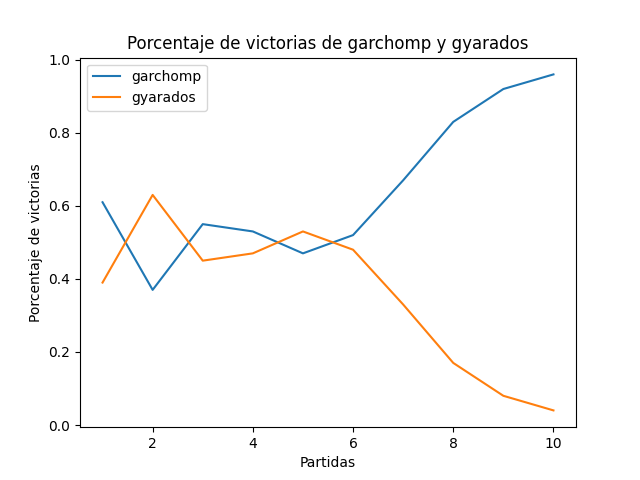
\includegraphics[width=0.7\textwidth]{figures/garchomp-vs-gyarados.png}
    \caption{Combate entre Garchomp y Gyarados.}
    \label{fig:turn}
\end{figure}

\begin{figure}[H]
    \centering
    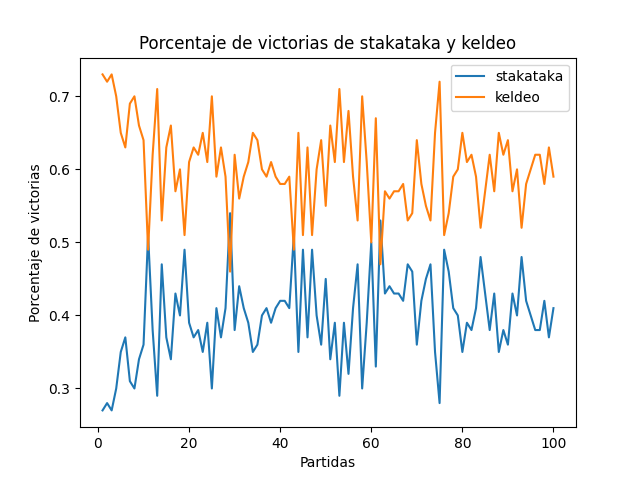
\includegraphics[width=0.7\textwidth]{figures/stakataka-vs-keldeo.png}
    \caption{Combate entre Stakataka y Keldeo.}
    \label{fig:turn}
\end{figure}

En ambas figuras se puede observar que la ia comienza eligiendo ataques de forma aleatoria hasta que encuentra uno que le permite ganar todas las partidas. De esta forma, se crea un balance entre ambos jugadores en el que uno gana siempre.

Hemos observado que al realizar el entrenamiento del agente global, existe un error que invierte el valor de las recompensas. Esto hace que el modelo tenga como objetivo perder. En la siguiente figura, la inteligencia artifial está jugando como el jugador 2, y vemos que solo tiene un porcentaje de victorias de aproximadamente 35%.

\begin{figure}[H]
    \centering
    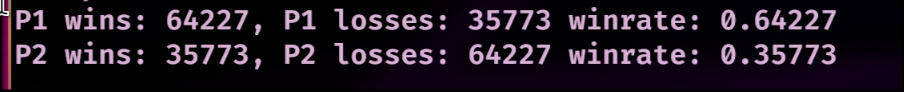
\includegraphics[width=0.9\textwidth]{figures/test_agente_global.jpeg}
    \caption{Combate entre Stakataka y Keldeo.}
    \label{fig:turn}
\end{figure}

\section{Posibles ampliaciones}

Además de solucionar el error presentado anteriormente, otras de las posibles mejoras para el proyecto incluyen utilizar más datos en el estado del juego, como por ejemplo las estadísticas de defensa y velocidad del pokémon. 

Una funcionalidad que no ha sido posible implementar es utilizar el motor gráfico del Pokémon Showdown para poder visualizar las batallas, e incluso probar los modelos contra jugadores reales online.


\end{document}
